% !TeX root = main.tex
\documentclass[twoside,a4paper,12pt]{article}


\usepackage[utf8]{inputenc}
\usepackage[english,polish]{babel} %\foreignlanguage{english}{eng. \textit{english}}
\usepackage{polski}
\usepackage{helvet}
\usepackage{graphicx}
\usepackage{color}
\usepackage{geometry}
\usepackage{url}
\usepackage[hidelinks]{hyperref}
\usepackage{minted}
\usepackage{amsmath}

\geometry{hmargin={2.5cm, 2cm}, height=10.0in}
\usepackage{epstopdf}

\usepackage{multicol}
\usepackage[toc,page]{appendix}
\usepackage{caption}
\usepackage{float}
\usepackage{enumitem}
\setlist{nosep}

\usepackage{emptypage}
\pretocmd{\section}{\cleardoublepage}{}{}

% !TeX root = ../main.tex
\newcommand{\setSupervisor}[1]{
    \newcommand{\supervisor}{#1}
}
\newcommand{\setFaculty}[1]{
    \newcommand{\faculty}{#1}
}
\newcommand{\setMajor}[1]{
    \newcommand{\major}{#1}
}

\newcommand{\setDepartment}[1]{
    \newcommand{\department}{#1}
}

\newcommand{\setReviewer}[1]{
    \newcommand{\reviewer}{#1}
}

\makeatletter
\renewcommand{\maketitle}{\begin{titlepage}
        
\includegraphics[height=37.5mm]{img/agh_nzw_a_pl_1w_wbr_cmyk}\\
        \rule{30mm}{0pt}
        {\large \textsf{\department}}\\
        \rule{\textwidth}{3pt}\\
        \rule[2ex]
        {\textwidth}{1pt}\\
        \vspace{7ex}
        \begin{center}
            {\LARGE \bf \textsf{Praca inżynierska}}\\
            \vspace{13ex}
            % --------------------------- IMIE I~NAZWISKO -------------------------------
            {\bf \Large \textsf{\@author}}\\
            \vspace{3ex}
            {\sf\small kierunek studiów:} {\bf\small \textsf{\faculty}}\\
            \vspace{1.5ex}
            \ifx\major\undefined\else\ifx\major\empty\else
                {\sf\small specjalność:} {\bf\small \textsf{\major}}\\
                \vspace{1.5ex}
            \fi\fi
            \vspace{8ex}
            %% ------------------------ TYTUL PRACY --------------------------------------
            {\bf \huge \textsf{\@title}}\\
            \vspace{14ex}
            %% ------------------------ OPIEKUN PRACY ------------------------------------
            {\Large Opiekun: \bf \textsf{\supervisor}}\\
            \vspace{22ex}
            {\large \bf \textsf{Kraków, \@date}}
        \end{center}
    \end{titlepage}%
}
\makeatother

\setminted[c]{frame=lines,
    framesep=2mm,
    baselinestretch=1.2,
    fontsize=\footnotesize,
    linenos}

\setminted[matlab]{frame=lines,
    framesep=2mm,
    baselinestretch=1.2,
    fontsize=\footnotesize,
    linenos}


\author{Tymon Woźniak}
\title{Implementacja i~testowanie efektywności detekcji wybranego algorytmu radaru pasywnego używającego sygnału Wi-Fi}
\date{2026}
\setDepartment{Wydział Informatyki, Elektroniki i~Telekomunikacji}
\setFaculty{Teleinformatyka}
\setMajor{}
\setSupervisor{prof. dr hab. inż. Tomasz Zieliński}
\setReviewer{}

\begin{document}
\pagestyle{empty}

\maketitle

% !TeX root = ../main.tex
%% =====  TEMATYKA I PROGRAM PRACY INŻYNIERSKIEJ ====

\newpage
\rightline{Kraków, 30 kwietnia 2026 r.}
\begin{center}
    {\bf Tematyka pracy inżynierskiej i~praktyki dyplomowej\\
        \makeatletter\@author\makeatother,
        studenta studiów pierwszego stopnia na kierunku teleinformatyka (nr albumu: 422842)}\\
\end{center}

\begin{center}
    Temat pracy inżynierskiej:\\
    \makeatletter
    {\bf \@title}\\
    \makeatother
\end{center}

\begin{tabular}{rl}
    Opiekun pracy:               & \supervisor \\
    Recenzent pracy:             & \reviewer \\
    Miejsce praktyki dyplomowej: & WIEiT AGH, Kraków \\
\end{tabular}

\begin{center}
    {\bf Program pracy inżynierskiej i~praktyki dyplomowej}
\end{center}

\begin{enumerate}
    \item Omówienie koncepcji i~zakresu pracy inżynierskiej z~opiekunem.
    \item Zebranie i~studium literatury z~zakresu pasywnej radiolokacji (PBR) oraz standardu transmisji Wi-Fi IEEE 802.11a (modulacja OFDM, estymacja kanału).
    \item Praktyka dyplomowa:
          \begin{itemize}
              \item zapoznanie się ze środowiskiem symulacyjnym MATLAB i~narzędziami przetwarzania sygnałów radarowych,
              \item implementacja modułów nadajnika Wi-Fi (ramka 802.11a Non-HT) oraz wielodrogowego kanału radiowego z~efektem Dopplera,
              \item opracowanie odbiornika pasywnego: synchronizacja Schmidl--Cox, demodulacja OFDM, estymacja kanału metodą Zero-Forcing, filtracja MTI oraz okienkowanie 2D Blackman--Harris.
          \end{itemize}
    \item Implementacja algorytmu koherentnego usuwania celów Coherent CLEAN oraz odbiornika korelacyjnego (funkcja wzajemnej niejednoznaczności CAF) jako metody odniesienia.
    \item Przeprowadzenie badań symulacyjnych efektywności detekcji radaru Wi-Fi: generacja map Range--Doppler (2D/3D), analiza przekrojów 1D, wyznaczenie charakterystyk $SNR_{\mathrm{out}} = f(SNR_{\mathrm{in}})$ oraz ocena odporności na zakłócenia i~wielodrogowość.
    \item Analiza porównawcza metody CIR i~CAF oraz ocena skuteczności algorytmu Coherent CLEAN w~scenariuszach wielocelowych.
    \item Opracowanie redakcyjne tekstu pracy inżynierskiej i~wniosków końcowych.
\end{enumerate}

\noindent
Termin oddania w~dziekanacie: \\[1cm]

\begin{center}
    \begin{tabular}{lcr}
        .............................................................. & ~~~ &
        ..............................................................                           \\
        (podpis kierownika katedry)                                    &     & (podpis opiekuna) \\
    \end{tabular}
\end{center}
\null
\newpage
\null
\newpage

\pagestyle{plain}
\linespread{1.3}
\selectfont

\newpage
\pagenumbering{roman}
\tableofcontents
\newpage
\thispagestyle{empty}
\mbox{}
\newpage

\pagenumbering{arabic}

% !TeX root = ../main.tex
\section{Wstęp}
\label{sec:introduction}

% ------------------------------------------------------------------------
% Cel i zakres pracy:
%   - implementacja toru radaru pasywnego (PBR) opartego na estymacji transmitancji kanału (CFR/CIR)
%   - analiza porównawcza dwóch generacji Wi-Fi: IEEE 802.11a (Legacy) oraz IEEE 802.11ax (Wi-Fi 6)
%   - ewaluacja w dwóch modelach propagacyjnych: syntetycznym oraz znormalizowanym TGax Model-B
% Motywacja:
%   - wszechobecność sygnałów Wi-Fi jako darmowych iluminatorów okazji
%   - przejście ze starszego 802.11a do powszechnego obecnie 802.11ax i implikacje radarowe
%   - konieczność weryfikacji algorytmów w realistycznym clutterze wielodrogowym (TGax)
% Teza i pytania badawcze:
%   - wpływ 4-krotnie dłuższego symbolu OFDM w 802.11ax na prędkość jednoznaczną (aliasing Dopplera)
%   - wpływ poszerzonej luki nośnych DC (3 podnośne) i jej interpolacji na wyciek widmowy
%   - odporność filtracji MTI i algorytmu Coherent CLEAN na gęsty clutter wielodrogowy TGax
% Układ pracy:
%   - krótki opis zawartości poszczególnych rozdziałów (1-6)
% ------------------------------------------------------------------------

\subsection{Cel i zakres pracy}
\label{subsec:intro_scope}

\subsection{Motywacja}
\label{subsec:intro_motivation}

\subsection{Teza i pytania badawcze}
\label{subsec:intro_thesis}

\subsection{Układ pracy}
\label{subsec:intro_structure}
% !TeX root = ../main.tex
\section{Radar Pasywny}
\label{sec:passive_radar}

% ------------------------------------------------------------------------
% Rozdział 2: Podstawy teoretyczne radaru pasywnego i sygnału Wi-Fi
% 2.1 Sygnał Wi-Fi 802.11 (ewolucja standardów, formaty ramek Non-HT i HE-SU)
% 2.2 Modulacja OFDM (podnośne, prefiks cykliczny CP, parametry symbolu)
% 2.3 Podstawy radaru pasywnego (geometria bistatyczna, bilans mocy, DPI, clutter)
% 2.4 Estymacja kanału (paradygmat CIR a funkcja CAF, estymator Zero-Forcing)
% 2.5 Filtracja ech stałych (filtr MTI w czasie wolnym, kompensacja luki DC)
% 2.6 Wyznaczanie mapy Range–Doppler (okno 2D Blackmana--Harrisa, IFFT/FFT)
% 2.7 Detekcja i ekstrakcja celów (algorytm Coherent CLEAN, próg szumu MAD)
% ------------------------------------------------------------------------

\subsection{Warstwa fizyczna standardu IEEE 802.11}
\label{subsec:wifi_signal}

Sieci WLAN zgodne z rodziną standardów IEEE 802.11 pracują w~nielicencjonowanych pasmach 2,4, 5 i~6~GHz, a~ich punkty dostępowe są rozmieszczone gęsto w~budynkach i~przestrzeni miejskiej. Z~punktu widzenia radaru pasywnego jest to szerokopasmowy iluminator okazjonalny o~małej mocy, przydatny przede wszystkim w~scenariuszach krótkozasięgowych \cite{colone2014,storrer2021,sorbianWykorzystanieSieciWifi2025}. W~pracy rozważono dwie warstwy fizyczne: Non-HT standardu IEEE 802.11a \cite{1999} oraz HE-SU standardu IEEE 802.11ax \cite{2021}. Obie wykorzystują modulację OFDM (podrozdział~\ref{subsec:ofdm_modulation}), lecz różnią się parametrami siatki czas--częstotliwość, zestawionymi w~tabeli~\ref{tab:wifi_params}. Pominięto warstwę MAC, kodowanie kanałowe i~przeplot, ponieważ odbiornik radarowy operuje bezpośrednio na symbolach konstelacji przypisanych do podnośnych.

\begin{table}[htbp]
    \centering
    \caption{Parametry warstwy fizycznej IEEE 802.11a i~802.11ax istotne dla przetwarzania radarowego \cite{1999,2021}}
    \label{tab:wifi_params}
    \small
    \begin{tabular}{|l|c|c|}
        \hline
        \textbf{Parametr} & \textbf{802.11a (Non-HT)} & \textbf{802.11ax (HE-SU, 20~MHz)} \\
        \hline
        Pasma częstotliwości & 5~GHz & 2,4 / 5 / 6~GHz \\
        Szerokości kanału & 20~MHz & 20 / 40 / 80 / 160~MHz \\
        Rozmiar FFT $N_{\mathrm{FFT}}$ & 64 & 256 \\
        Odstęp podnośnych $\Delta f$ & 312,5~kHz & 78,125~kHz \\
        Czas użyteczny symbolu $T_u$ & 3,2~$\mu$s & 12,8~$\mu$s \\
        Prefiks cykliczny $T_{\mathrm{CP}}$ & 0,8~$\mu$s & 0,8 / 1,6 / 3,2~$\mu$s \\
        Czas symbolu $T_{\mathrm{sym}}$ (dla $T_{\mathrm{CP}} = 0{,}8~\mu$s) & 4,0~$\mu$s & 13,6~$\mu$s \\
        Podnośne aktywne (danych + pilotowe) & 52 (48 + 4) & 242 (234 + 8) \\
        Podnośne zerowe w~centrum pasma (DC) & 1 & 3 \\
        Podnośne ochronne (lewe / prawe) & 6 / 5 & 6 / 5 \\
        Pola treningowe preambuły & L-STF, L-LTF & L-STF, L-LTF, HE-STF, HE-LTF \\
        Modulacje pola danych & BPSK -- 64-QAM & BPSK -- 1024-QAM \\
        \hline
    \end{tabular}
\end{table}

Każda transmisja ma postać ramki PPDU (ang. \textit{PHY Protocol Data Unit}), złożonej z~preambuły i~pola danych. W~standardzie 802.11a preambuła obejmuje krótkie pole treningowe L-STF (8~$\mu$s), długie pole treningowe L-LTF (8~$\mu$s) oraz pole sygnalizacyjne L-SIG (4~$\mu$s) \cite{1999}. W~ramce HE-SU sekwencję tę zachowano dla kompatybilności wstecznej i~uzupełniono o~pola RL-SIG, HE-SIG-A, HE-STF i~HE-LTF \cite{2021}. Pola treningowe (L-LTF oraz HE-LTF) zawierają zdefiniowane w~standardzie sekwencje o~stałej amplitudzie symboli ($|X_k| = 1$). Dzięki temu energia nadawana na każdej podnośnej jest jednakowa, co ułatwia odbiornikowi komunikacyjnemu precyzyjne wyznaczenie transmitancji kanału. Pole danych przenosi natomiast losowe symbole danych o~modulacji wynikającej z~wybranego schematu MCS (ang. \textit{Modulation and Coding Scheme}) -- od BPSK i~QPSK po modulacje kwadraturowe wyższych rzędów: 16-QAM i~64-QAM w~802.11a oraz do 1024-QAM w~802.11ax.

Podział ramki na preambułę i~pole danych otwiera dwie drogi pozyskania sygnału odniesienia w~radarze pasywnym:
\begin{itemize}
    \item \textbf{Wykorzystanie wyłącznie preambuły} -- sekwencje treningowe są znane odbiornikowi z~góry i~nie wymagają demodulacji. Podejście to daje jednak tylko jedną estymatę kanału na całą ramkę. W~konsekwencji częstotliwość próbkowania w~osi prędkości zależy od nieregularnych przerw między pakietami w~sieci \cite{zotero-item-46}.
    \item \textbf{Wykorzystanie pola danych} -- pojedyncza ramka zawiera od kilkudziesięciu do kilkuset kolejnych symboli OFDM. Zapewnia to gęstą i~równomierną siatkę próbkowania w~czasie wolnym \cite{braun2014}, kosztem konieczności poprawnej demodulacji nadanych symboli w~kanale referencyjnym.
\end{itemize}
Eksperymenty opisane w~literaturze potwierdzają, że włączenie symboli danych znacząco poprawia wykrywalność celów w~porównaniu z~przetwarzaniem wyłącznie sygnałów pilotowych \cite{wypich2026}. Z~tego względu w~opracowanym symulatorze (rozdział~\ref{sec:radar_implementation}) do przetwarzania radarowego wykorzystano pole danych.

\begin{figure}[H]
    \centering
    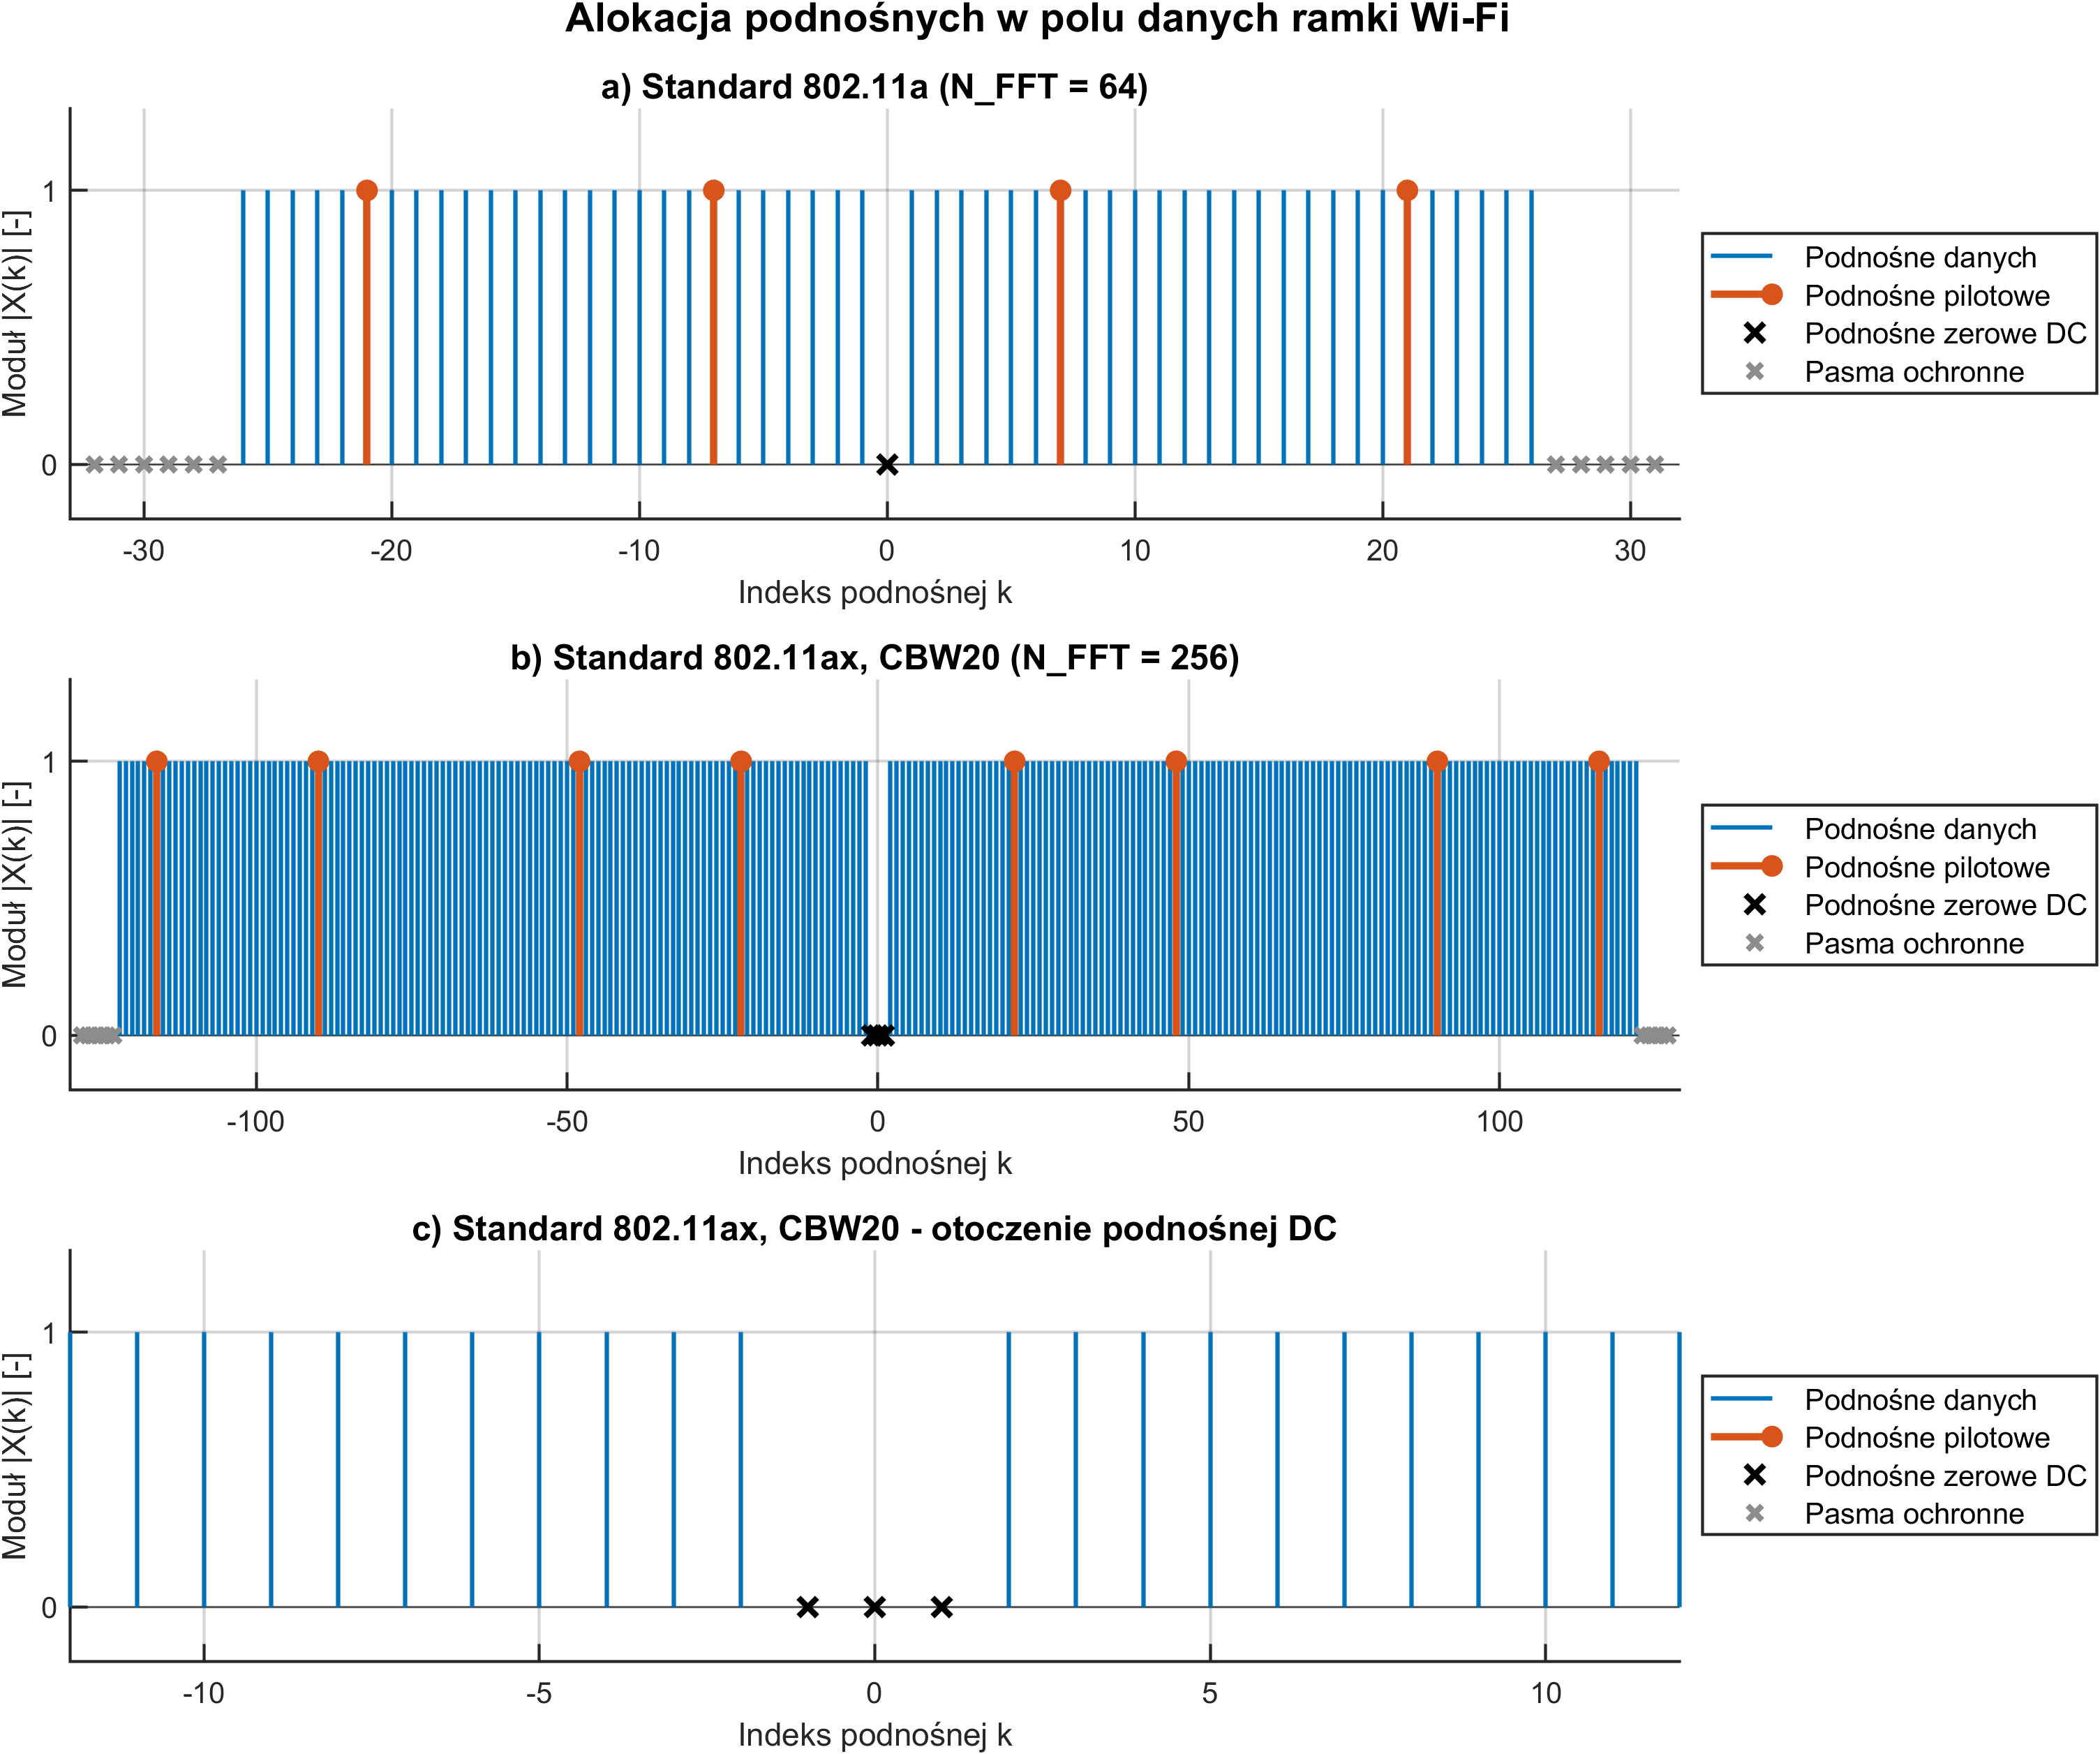
\includegraphics[width=\textwidth]{img/ch2_theory/rys_2_1_alokacja_podnosnych.png}
    \caption{Alokacja podnośnych w~polu danych: a)~802.11a, b)~802.11ax przy szerokości kanału 20~MHz, c)~powiększenie otoczenia podnośnej DC w~802.11ax. Podnośne zerowe zaznaczono krzyżykami na poziomie zera}
    \label{fig:subcarrier_allocation}
\end{figure}

Rozkład podnośnych w~paśmie przedstawiono na rysunku~\ref{fig:subcarrier_allocation}. W~standardzie 802.11a aktywne są 52 z~64 podnośnych, a~w~802.11ax przy szerokości kanału 20~MHz wykorzystywane są 242 z~256 podnośnych. Podnośne pilotowe służą odbiornikowi komunikacyjnemu do śledzenia fazy i~zajmują ściśle określone pozycje w~siatce częstotliwościowej. Skrajne podnośne pozostawiono puste jako pasma ochronne, ograniczające emisję poza przydzielonym kanałem. Wyzerowano również podnośną centralną $k = 0$ (w~802.11ax wraz z~sąsiednimi $k = \pm 1$, co pokazano na rysunku~\ref{fig:subcarrier_allocation}c). W~odbiornikach radiowych na zerowej częstotliwości pośredniej naturalnie powstaje silny prążek zakłóceń od napięcia stałego oraz wewnętrznego oscylatora -- brak transmisji na tych podnośnych zapobiega więc zniekształceniu danych.

Alokacja podnośnych przenosi się bezpośrednio na właściwości wyznaczanej mapy odległość--prędkość:
\begin{itemize}
    \item Pasma ochronne ograniczają efektywnie zajęte pasmo do ok.~16,6~MHz w~802.11a oraz 19,1~MHz w~802.11ax, co determinuje rozdzielczość odległościową (podrozdział~\ref{subsec:pbr_fundamentals}).
    \item Wyzerowane podnośne DC tworzą nieciągłość (dziurę) w~środku widma, co po transformacji Fouriera podnosi tło listków bocznych w~osi odległości \cite[rozdz.~3.3.8]{braun2014}. Problem ten rozwiązuje interpolacja opisana w~podrozdziale~\ref{subsec:clutter_filtering}.
    \item Zmienna amplituda punktów konstelacji QAM w~polu danych powoduje wzmocnienie szumu estymaty kanału przy dzieleniu Zero-Forcing, co szczegółowo przeanalizowano w~podrozdziale~\ref{subsec:channel_estimation} i~zbadano w~podrozdziale~\ref{subsec:sim_mcs_noise_enhancement}.
    \item Czterokrotnie mniejszy odstęp podnośnych w~802.11ax wydłuża czas trwania symbolu z~4,0 do 13,6~$\mu$s. Zwiększa to zasięg jednoznaczny, lecz proporcjonalnie obniża maksymalną jednoznaczną prędkość radaru (podrozdział~\ref{subsec:pbr_fundamentals}).
\end{itemize}

\subsection{Modulacja OFDM}
\label{subsec:ofdm_modulation}

\subsection{Podstawy radaru pasywnego}
\label{subsec:pbr_fundamentals}

\subsection{Estymacja kanału}
\label{subsec:channel_estimation}

\subsection{Filtracja ech stałych}
\label{subsec:clutter_filtering}

\subsection{Wyznaczanie mapy Range--Doppler}
\label{subsec:range_doppler_map}

\subsection{Detekcja i ekstrakcja celów}
\label{subsec:target_detection_extraction}

% !TeX root = ../main.tex
\section{Implementacja radaru}
\label{sec:radar_implementation}

% ------------------------------------------------------------------------
% Rozdział 3: Implementacja poszczególnych bloków radaru w środowisku MATLAB
% 3.1 Środowisko symulacyjne MATLAB i toolboxy (WLAN Toolbox, Communications Toolbox, wkład własny)
% 3.2 Implementacja kanału (step2_channel.m, kanały TGax A/C/E, symulacja celów ruchomych i opóźnień)
% 3.3 Implementacja odbiornika (step3_receiver.m, demodulacja OFDM, Zero-Forcing, filtr MTI, interpolacja DC)
% 3.4 Implementacja interpretera (step4_interpreter.m, okno Blackmana--Harrisa, periodogram 2D, Coherent CLEAN, osie fizyczne)
% ------------------------------------------------------------------------

\subsection{Środowisko symulacyjne MATLAB i toolboxy}
\label{subsec:matlab_environment_toolboxes}

\subsection{Implementacja kanału}
\label{subsec:channel_implementation}

\subsection{Implementacja odbiornika}
\label{subsec:receiver_implementation}

\subsection{Implementacja interpretera}
\label{subsec:interpreter_implementation}

% !TeX root = ../main.tex
\section{Badania symulacyjne}
\label{sec:simulation_results}

% ------------------------------------------------------------------------
% Rozdział 4: Badania symulacyjne efektywności detekcji radaru
% 4.1 Scenariusze testowe (parametryzacja, stała moc AP 100 mW EIRP, degradacja szumowa 9 dB dla 160 MHz)
% 4.2 Rozdzielczość odległościowa a szerokość pasma (E1: 20, 40, 80, 160 MHz)
% 4.3 Długość symbolu OFDM a prędkość jednoznaczna (E2: 802.11a vs 802.11ax, aliasing Dopplera)
% 4.4 Wpływ rzędu modulacji MCS i poziomu szumu na estymację ZF (E3: wzmocnienie szumu zeta_ZF, kontrast PNFR)
% 4.5 Tłumienie stacjonarnego clutteru (E4: modele TGax A, C, E, filtr MTI w czasie wolnym)
% 4.6 Skuteczność algorytmu Coherent CLEAN (E5: duża dynamika mocy >30 dB, odsłanianie celów słabych, adaptacyjny próg MAD, Monte Carlo)
% ------------------------------------------------------------------------

\subsection{Scenariusze testowe}
\label{subsec:sim_scenarios}

\subsection{Rozdzielczość odległościowa a szerokość pasma}
\label{subsec:sim_bandwidth_resolution}

\subsection{Długość symbolu OFDM a prędkość jednoznaczna}
\label{subsec:sim_doppler_aliasing}

\subsection{Wpływ rzędu modulacji MCS i poziomu szumu na estymację ZF}
\label{subsec:sim_mcs_noise_enhancement}

\subsection{Tłumienie stacjonarnego clutteru}
\label{subsec:sim_clutter_suppression}

\subsection{Skuteczność algorytmu Coherent CLEAN}
\label{subsec:sim_clean_performance}

% !TeX root = ../main.tex
\section{Wnioski}
\label{sec:conclusion}

% ------------------------------------------------------------------------
% Rozdział 5: Wnioski i podsumowanie
% 5.1 Podsumowanie uzyskanych wyników (wnioski z implementacji i badań E1-E5 / Monte Carlo)
% 5.2 Ograniczenia metody i kierunki rozwoju (aliasing ax, bilans mocy AP, multi-frame CPI, pomiary SDR/CSI)
% ------------------------------------------------------------------------

\subsection{Podsumowanie uzyskanych wyników}
\label{subsec:conclusion_summary}

\subsection{Ograniczenia metody i kierunki rozwoju}
\label{subsec:conclusion_limitations_and_future_work}


\newpage
\addcontentsline{toc}{section}{Literatura}
\bibliographystyle{plain}
\nocite{*}
\bibliography{bibliography}

\newpage
\addcontentsline{toc}{section}{Spis rysunków}
\listoffigures

\newpage
\addcontentsline{toc}{section}{Spis tabel}
\listoftables

\end{document}
